\chapter{Pruebas}\label{cap:pruebas}

Este capítulo describe cómo se ha comprobado que el sistema funciona y que cumple los requisitos del Capítulo~\ref{cap:analisis}. Las pruebas se han organizado en cuatro niveles, de menor a mayor alcance:

\begin{enumerate}
    \item \textbf{Pruebas automáticas del backend}, que comprueban la lógica de negocio y la seguridad de la API clase a clase.
    \item \textbf{Pruebas de simulación del seguimiento en tiempo real}, con un simulador propio que imita a varios cofrades compartiendo su ubicación.
    \item \textbf{Pruebas en directo} con el sistema desplegado en el servidor, el simulador enviando las ubicaciones de los cofrades y la aplicación en un dispositivo real.
    \item \textbf{Pruebas manuales de aceptación} de cada caso de uso sobre la aplicación.
\end{enumerate}

Por último, se resumen los errores detectados durante las pruebas y su corrección.

\section{Pruebas automáticas del backend}\label{sec:pruebasBackend}

El backend cuenta con un conjunto de pruebas automáticas escritas con JUnit~5~\cite{junit} y Mockito~\cite{mockito}, que se ejecutan con el comando \texttt{./mvnw test}. Se distinguen dos tipos:

\begin{itemize}
    \item \textbf{Pruebas unitarias de la capa de servicio y de las utilidades}. Cada prueba comprueba una sola clase, sustituyendo sus dependencias (repositorios, otros servicios, el envío de correo o de notificaciones \emph{push}) por objetos simulados con Mockito. Así se verifica la lógica de negocio sin necesidad de una base de datos: las reglas de autorización por rol y por ciudad, los cambios de estado, la caducidad de los códigos de acceso, el cálculo de la estela, etc.
    \item \textbf{Pruebas de la API} (\texttt{SeguridadApiTest}), con Spring Boot Test y MockMvc. Envían peticiones HTTP a los controladores, sin arrancar un servidor real, para comprobar qué rutas son públicas y cuáles exigen sesión, cómo se traducen los errores a códigos HTTP y que se validan los datos de entrada.
\end{itemize}

La Tabla~\ref{tab:pruebasBackend} recoge las clases de prueba, el número de pruebas de cada una y lo que comprueban. En total son \textbf{217 pruebas}, y todas se superan.

\begin{table}[H]
\centering
\small
\renewcommand{\arraystretch}{1.2}
\begin{tabular}{|p{4.6cm}|c|p{8.4cm}|}
\hline
\textbf{Clase de prueba} & \textbf{Pruebas} & \textbf{Qué comprueba} \\
\hline
\texttt{SeguridadApiTest} & 28 & Rutas públicas y protegidas, tokens falsos o ausentes, datos personales no públicos, traducción de errores a códigos HTTP (404, 403, 401, 409, 410) y validación de los datos de entrada. \\
\hline
\texttt{PosicionActualServiceTest} & 20 & Envío de ubicaciones por los cofrades: descarte de las que están a más de 50~m del recorrido, rechazo de cofrades de otra cofradía y de códigos revocados o caducados, posición actual y estela de la procesión, que nunca retrocede. \\
\hline
\texttt{MiembroJuntaCofradiaServiceTest} & 24 & Autorización de la Junta (miembro activo, Junta activa, contraseña provisional ya cambiada, misma ciudad), alta con contraseña provisional y correo de bienvenida, reenvío de la invitación y solicitudes de reactivación. \\
\hline
\texttt{AdministradorServiceTest} & 18 & Alta del primer administrador con el secreto de despliegue, gestión de administradores y de su perfil, correos duplicados. \\
\hline
\texttt{AuthServiceTest} & 17 & Inicio de sesión con correo y contraseña, inicio de sesión del cofrade con código (emitido, validado, revocado, caducado, de cofradía desactivada) y cambio de contraseña. \\
\hline
\texttt{ProcesionServiceTest} & 14 & Alta y edición de procesiones, recorrido único por procesión, autorización por ciudad, cambios de estado con su notificación y cancelación. \\
\hline
\texttt{GeometriaRutaTest} & 13 & Proyección de una ubicación sobre el recorrido para calcular cuánto ha avanzado la procesión, incluidos los recorridos que salen y vuelven al mismo templo. \\
\hline
\texttt{CofradiaServiceTest}, \texttt{CiudadServiceTest}, \texttt{JuntaCofradiasServiceTest}, \texttt{PasoServiceTest}, \texttt{EventoServiceTest}, \texttt{InformacionCiudadServiceTest} & 32 & Gestión del contenido por la Junta y el administrador: autorización por rol y por ciudad, elementos activos e inactivos, una Junta por ciudad, borrado con datos asociados y que el listado de eventos no incluya las procesiones. \\
\hline
\texttt{NotificacionServiceTest} & 10 & Notificaciones manuales (prioridad obligatoria, solo la Junta de la ciudad) y automáticas de inicio y fin. \\
\hline
\texttt{HorarioEventosTest}, \texttt{CambioEstadoAutomaticoServiceTest} & 15 & Cambio automático de estado al llegar la hora de inicio y de fin, y cambios manuales que contradicen el horario. \\
\hline
\texttt{GpxParserTest}, \texttt{RecorridoServiceTest}, \texttt{RecorridoPuntoRutaServiceTest}, \texttt{AutorizacionRecorridoServiceTest} & 32 & Lectura de archivos GPX (orden de prioridad, máximo de 300 puntos, archivos no válidos y protección frente a ataques XXE), importación y borrado de recorridos y marcado de puntos de interés. \\
\hline
\texttt{JwtServiceTest}, \texttt{CodigoAccesoServiceTest}, \texttt{DispositivoPushServiceTest}, \texttt{ValidacionImagenTest} & 22 & Tokens manipulados, firmados con otra clave o caducados, generación de códigos de acceso únicos, registro de dispositivos para \emph{push} y validación de las direcciones de imagen. \\
\hline
\textbf{Total} & \textbf{217} & \\
\hline
\end{tabular}
\caption{Pruebas automáticas del backend}
\label{tab:pruebasBackend}
\end{table}

\subsection{Cobertura}

La cobertura de las pruebas se ha medido con JaCoCo~\cite{jacoco}, que genera un informe en \texttt{target/site/jacoco} al ejecutar las pruebas. La Tabla~\ref{tab:cobertura} muestra el resultado por paquete.

\begin{table}[H]
\centering
\renewcommand{\arraystretch}{1.2}
\begin{tabular}{|l|c|c|}
\hline
\textbf{Paquete} & \textbf{Instrucciones} & \textbf{Ramas} \\
\hline
\texttt{util} (GPX y geometría del recorrido) & 99\,\% & 95\,\% \\
\hline
\texttt{security} (JWT y filtro de autenticación) & 98\,\% & 75\,\% \\
\hline
\texttt{model} & 81\,\% & 50\,\% \\
\hline
\texttt{exception} & 79\,\% & 83\,\% \\
\hline
\texttt{service} (lógica de negocio) & 77\,\% & 78\,\% \\
\hline
\texttt{controller} & 14\,\% & 14\,\% \\
\hline
\textbf{Total} & \textbf{73\,\%} & \textbf{77\,\%} \\
\hline
\end{tabular}
\caption{Cobertura de las pruebas automáticas del backend}
\label{tab:cobertura}
\end{table}

El esfuerzo se ha concentrado en la lógica de negocio y en la seguridad, que es donde un error tiene más consecuencias: la geometría del recorrido y el análisis de los GPX están cubiertos casi por completo, y la capa de servicio en más de tres cuartas partes. La baja cobertura de los controladores se debe a que estos se limitan a recibir la petición, llamar al servicio y devolver la respuesta, sin lógica propia; sus rutas de seguridad y de errores se comprueban en \texttt{SeguridadApiTest}, pero no se ha escrito una prueba HTTP para cada \emph{endpoint}.

\section{Pruebas de simulación del seguimiento en tiempo real}\label{sec:simulador}

El seguimiento de una procesión en tiempo real (RF-18, RF-24 y RF-25) no se puede probar a fondo con pruebas automáticas, porque depende de que varias personas compartan su ubicación a la vez mientras recorren las calles. Para probarlo sin salir a la calle con varios móviles se ha desarrollado un \textbf{simulador de procesiones}, un programa en Node.js incluido en el repositorio (\texttt{herramientas/simulador-procesion}).

El simulador hace lo mismo que la aplicación del cofrade: inicia sesión con un código de acceso y envía ubicaciones a la API, pero por varios cofrades virtuales repartidos a lo largo del cortejo, de la cabeza a la cola, que avanzan por el recorrido real de la procesión (el GPX importado). Permite configurar el número de cofrades, la longitud del cortejo, la velocidad de la procesión, un factor para acelerar el tiempo, el error típico del GPS y una proporción de ubicaciones erróneas, alejadas del recorrido. En cada ronda muestra cuántas ubicaciones ha aceptado y descartado el backend, y la estela que este calcula, que es lo que ve el ciudadano en el mapa.

La Tabla~\ref{tab:escenariosSimulador} recoge los escenarios probados con el simulador.

\begin{table}[H]
\centering
\small
\renewcommand{\arraystretch}{1.2}
\begin{tabular}{|p{3.2cm}|p{6cm}|p{4.8cm}|}
\hline
\textbf{Escenario} & \textbf{Qué se comprueba} & \textbf{Requisitos} \\
\hline
Seguimiento normal & La estela avanza en el mapa sin saltos y la cola va por detrás de la cabeza. & RF-16, RF-18, RF-24, RNF-05 \\
\hline
Ubicaciones erróneas & Con un 30\,\% de ubicaciones alejadas del recorrido, ninguna se guarda y el mapa no da saltos. & RF-25 \\
\hline
Recorrido circular & En una procesión que sale y vuelve al mismo templo, la estela no aparece completa al empezar. & RF-18 \\
\hline
Fin de la procesión & Al finalizar la procesión, el backend deja de aceptar ubicaciones y el simulador se detiene. & RF-24, RF-35 \\
\hline
Código revocado o caducado & Al revocar el código de acceso durante la simulación, el backend rechaza las ubicaciones y se informa del motivo. & RF-24, RF-31 \\
\hline
\end{tabular}
\caption{Escenarios probados con el simulador de procesiones}
\label{tab:escenariosSimulador}
\end{table}

En todos los escenarios el sistema se comportó como se esperaba. La Figura~\ref{fig:consolaSimulador} muestra la salida del simulador durante una de las pruebas: en cada ronda indica cuántas ubicaciones ha guardado y descartado el backend, el tramo del recorrido que ocupa la procesión (de la cola a la cabeza) y el número de ubicaciones activas. Las ubicaciones erróneas que genera el simulador aparecen como descartadas, y la estela avanza de forma continua sin retroceder.

\begin{figure}[H]
    \centering
    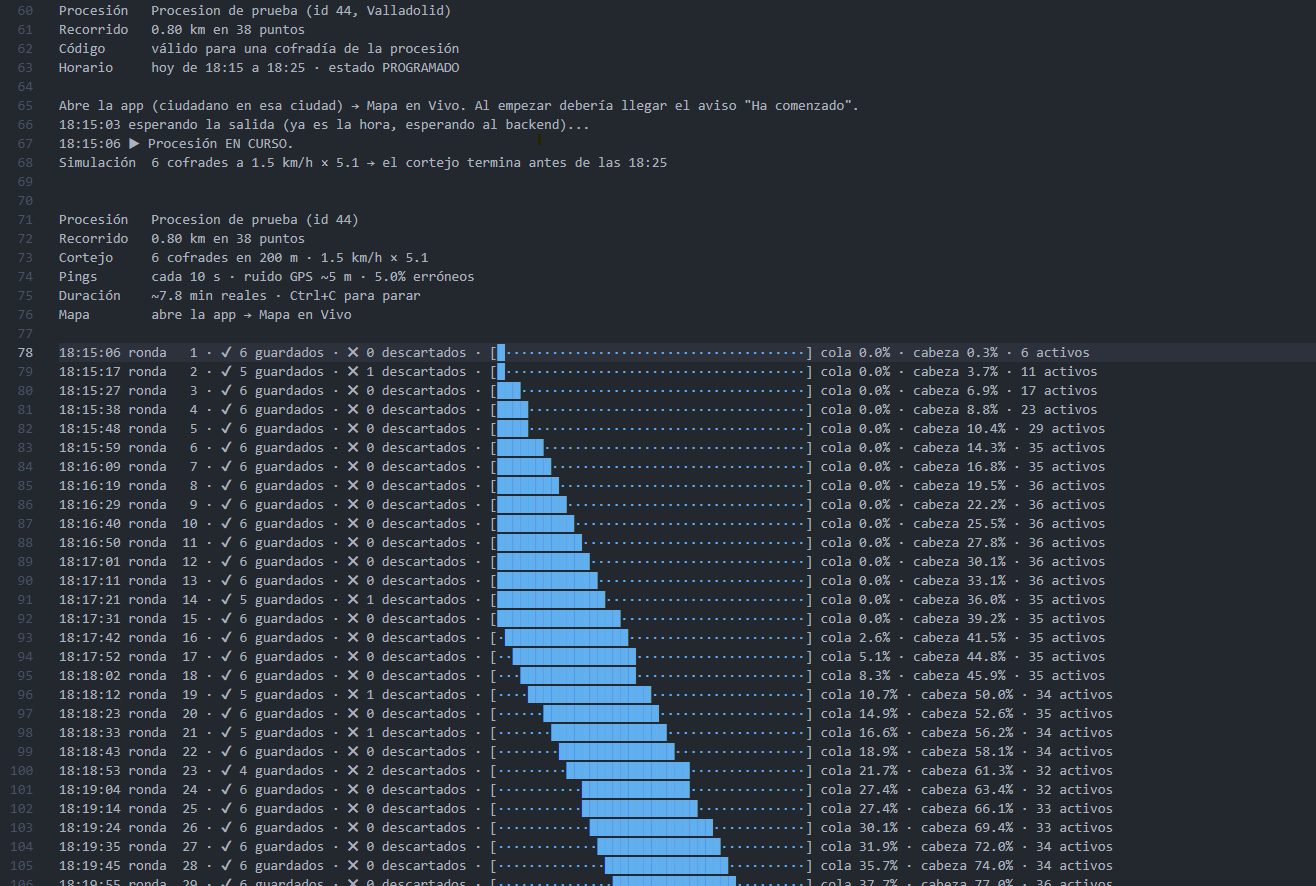
\includegraphics[width=\textwidth]{imagenes/consola_una_proecsion.png}
    \caption{Salida del simulador de procesiones durante una prueba}
    \label{fig:consolaSimulador}
\end{figure}

\section{Pruebas en directo}\label{sec:pruebasDirecto}

Además de las simulaciones, se han realizado pruebas con el sistema completo en condiciones reales: el backend desplegado en el servidor de la Universidad (Apéndice~\ref{cap:manual_despliegue}), las notificaciones enviadas por Expo y la aplicación ejecutándose en un dispositivo físico. En estas pruebas las ubicaciones de los cofrades no se enviaron desde varios móviles, sino con el simulador de la Sección~\ref{sec:simulador}, lanzado desde un programa auxiliar; el dispositivo físico se utilizó como ciudadano, para seguir las procesiones en el Mapa en Vivo y recibir las notificaciones.

\subsection{Procesión de prueba}

La primera prueba en directo se realizó el 26 de octubre de 2026 con una procesión de prueba de 10 minutos de duración, programada a las 18:15. Como el formulario de la aplicación solo permite elegir los días de la Semana Santa, se preparó con un programa auxiliar (\texttt{prueba-hoy.mjs}, junto al simulador) que traslada la procesión al día de la prueba, comprueba el código de acceso antes de la hora y lanza el simulador cuando el backend la pone en curso. Se comprobó:

\begin{itemize}
    \item que el backend cambiaba la procesión a \emph{en curso} por sí solo al llegar la hora de inicio, y que llegaba al dispositivo la notificación \emph{push} de inicio (RF-35, RF-36, RNF-08);
    \item que la procesión aparecía en el Mapa en Vivo sin que el ciudadano tuviera que seleccionarla, y que su estela avanzaba a medida que se recibían las ubicaciones (RF-16, RF-18);
    \item que se descartaban las ubicaciones erróneas (RF-25);
    \item que al llegar la hora de fin el backend la finalizaba, enviaba la notificación de fin y dejaba de aceptar ubicaciones (RF-24, RF-35).
\end{itemize}

La prueba se completó sin incidencias. La Figura~\ref{fig:pruebaUnaProcesion} muestra la procesión en el Mapa en Vivo, con la parte del recorrido ya ocupada por el cortejo marcada en verde, y las notificaciones de inicio y de fin recibidas en el dispositivo con 10 minutos de diferencia.

\begin{figure}[H]
    \centering
    \begin{subfigure}[b]{0.32\textwidth}
        \centering
        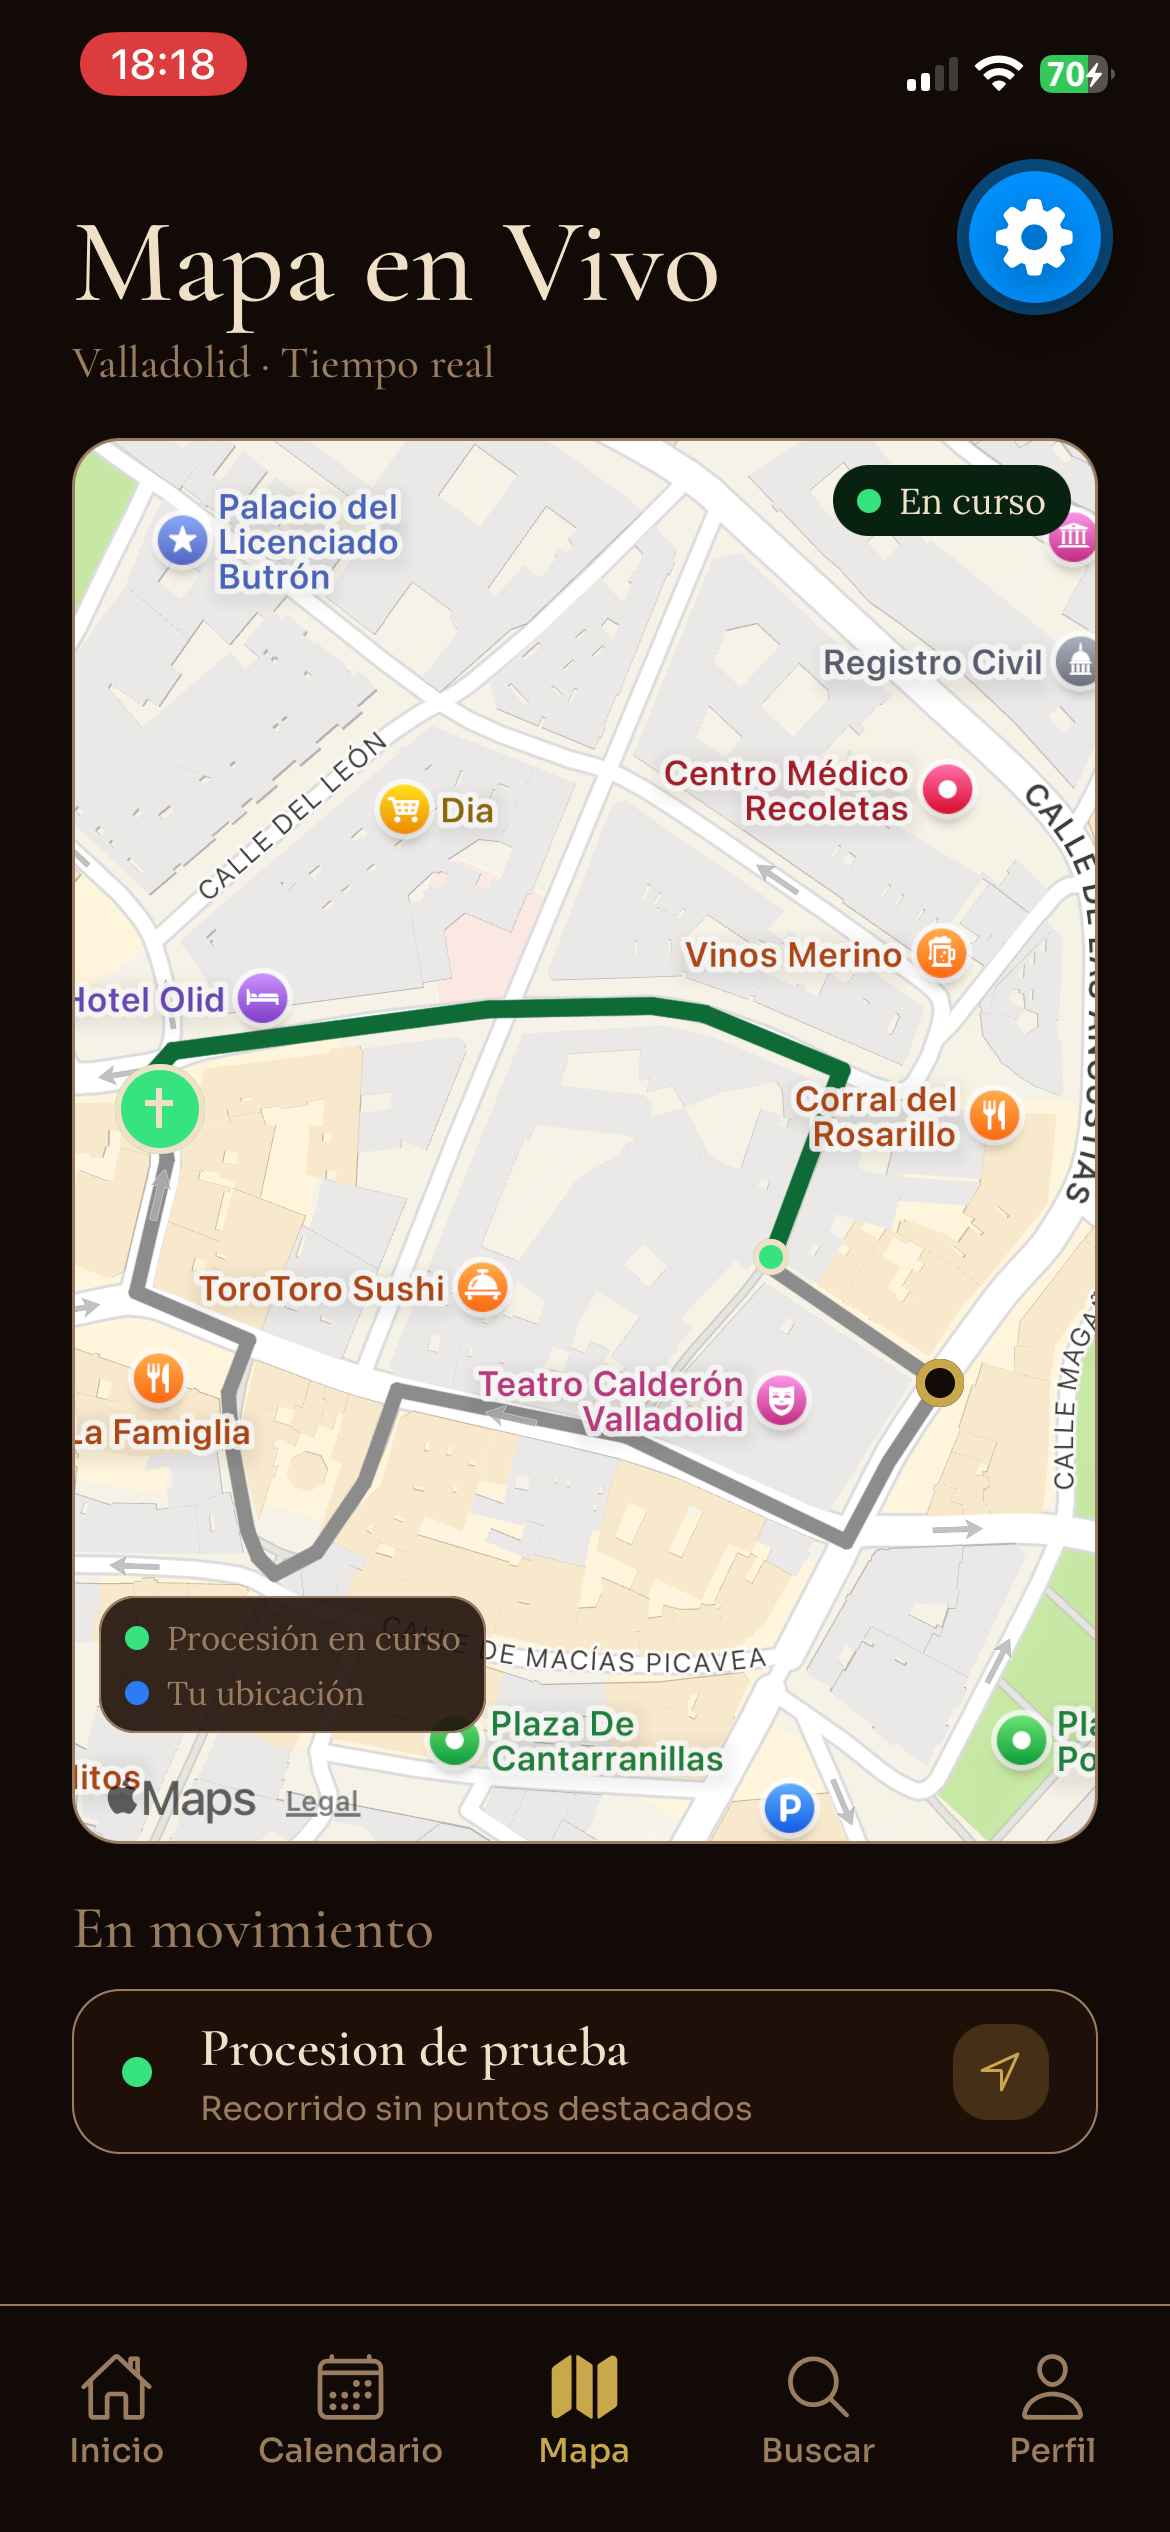
\includegraphics[width=\textwidth]{imagenes/una_procesion_activa.PNG}
        \caption{Mapa en Vivo}
    \end{subfigure}
    \hfill
    \begin{subfigure}[b]{0.62\textwidth}
        \centering
        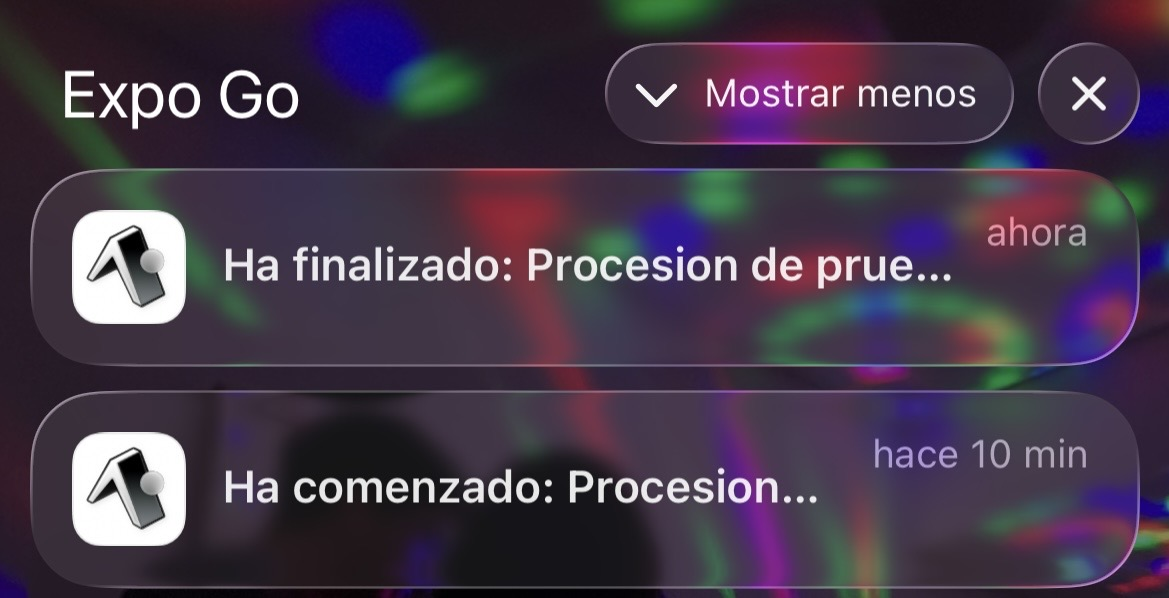
\includegraphics[width=\textwidth]{imagenes/notficacones.jpg}
        \caption{Notificaciones de inicio y de fin}
    \end{subfigure}
    \caption{Prueba en directo con una procesión}
    \label{fig:pruebaUnaProcesion}
\end{figure}

\subsection{Varias procesiones simultáneas}

Durante la Semana Santa es habitual que haya varias procesiones en la calle a la vez, a menudo con recorridos que comparten calles. Para comprobar que el sistema las distingue correctamente, el 28 de octubre de 2026 se realizó una segunda prueba en directo con tres procesiones de 10 minutos que salían con 3 minutos de diferencia, de forma que entre el minuto 6 y el 10 de la prueba las tres estaban en curso a la vez. Se utilizaron tres recorridos reales del centro de Valladolid, cortos y con calles en común, importados desde sus archivos GPX (Tabla~\ref{tab:pruebaSimultanea}).

\begin{table}[H]
\centering
\small
\renewcommand{\arraystretch}{1.2}
\begin{tabular}{|p{1.2cm}|p{4.6cm}|p{4.6cm}|p{2.6cm}|}
\hline
 & \textbf{Recorrido} & \textbf{Cofradía} & \textbf{Horario} \\
\hline
P1 & Ofrecimiento de los Dolores (0,9\,km) & Santa Vera Cruz & H a H+10 \\
\hline
P2 & Soledad (0,8\,km) & Nuestra Señora de las Angustias & H+3 a H+13 \\
\hline
P3 & Cristo de la Luz (1\,km) & Santísimo Cristo de la Luz & H+6 a H+16 \\
\hline
\end{tabular}
\caption{Procesiones de la prueba de procesiones simultáneas}
\label{tab:pruebaSimultanea}
\end{table}

La prueba se preparó con otro programa auxiliar (\texttt{prueba-varias.mjs}) que, con las credenciales de la Junta de Cofradías, importa los tres recorridos, crea las procesiones para el día de la prueba, emite un código de acceso para cada cofradía y, cuando el backend pone cada procesión en curso, lanza un simulador para ella con cinco cofrades virtuales. Al terminar, el mismo programa elimina las procesiones y los recorridos de prueba. Se comprobó:

\begin{itemize}
    \item que el backend ponía en curso y finalizaba cada procesión a su hora, de forma independiente, y que llegaban al dispositivo las seis notificaciones \emph{push}, una de inicio y otra de fin por cada procesión (RF-35, RF-36, RNF-08);
    \item que el Mapa en Vivo mostraba las procesiones en curso a medida que salían, y las tres a la vez durante el tramo en que coincidían, cada una con su propia estela (RF-16, RF-18);
    \item que las ubicaciones de los cofrades de una procesión no alteraban la estela de las demás, aunque sus recorridos compartieran calles;
    \item que el código de una cofradía no permitía enviar ubicaciones a una procesión en la que esta no participa (RF-24).
\end{itemize}

Las tres procesiones se siguieron correctamente de principio a fin, sin que ninguna estela se mezclara con la de otra ni retrocediera, y cada una desapareció del Mapa en Vivo al finalizar.

La Figura~\ref{fig:pruebaVariasProcesiones} muestra el momento en que las tres procesiones estaban en curso a la vez: en la pantalla de inicio aparecen las tres en ``En curso ahora'', junto al aviso de que acaba de comenzar la tercera, y en el Mapa en Vivo cada una se representa con su propia estela. La Figura~\ref{fig:consolaVariasProcesiones} recoge la salida del programa durante ese mismo tramo, con las rondas de las tres procesiones intercaladas.

\begin{figure}[H]
    \centering
    \begin{subfigure}[b]{0.4\textwidth}
        \centering
        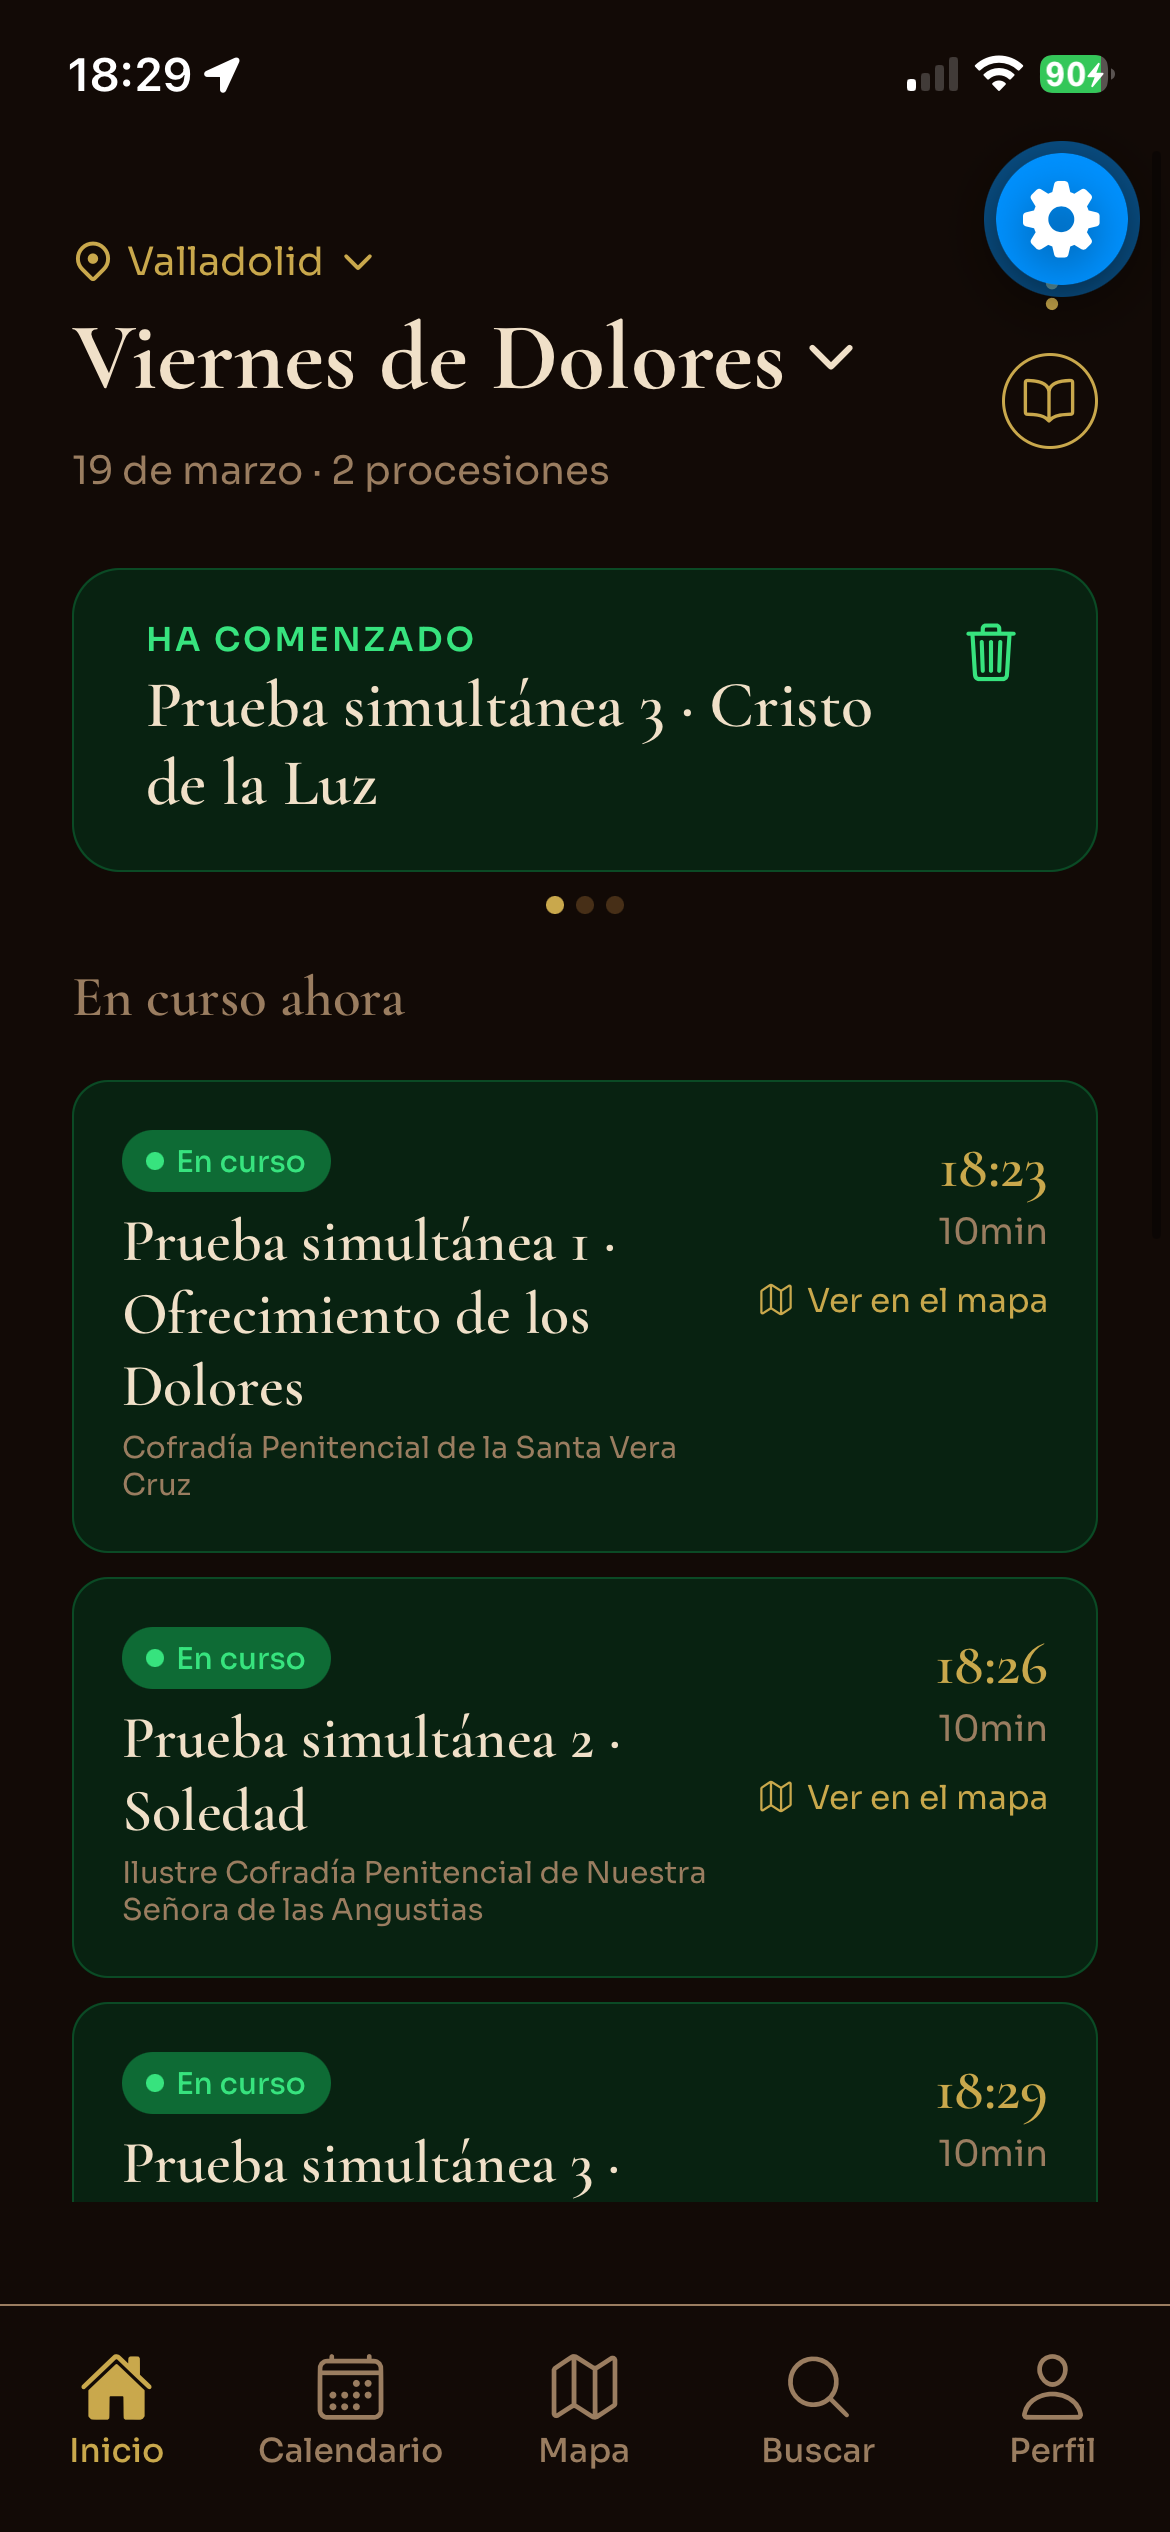
\includegraphics[width=\textwidth]{imagenes/inicio_variasProcesiones.PNG}
        \caption{Pantalla de inicio}
    \end{subfigure}
    \hspace{1cm}
    \begin{subfigure}[b]{0.4\textwidth}
        \centering
        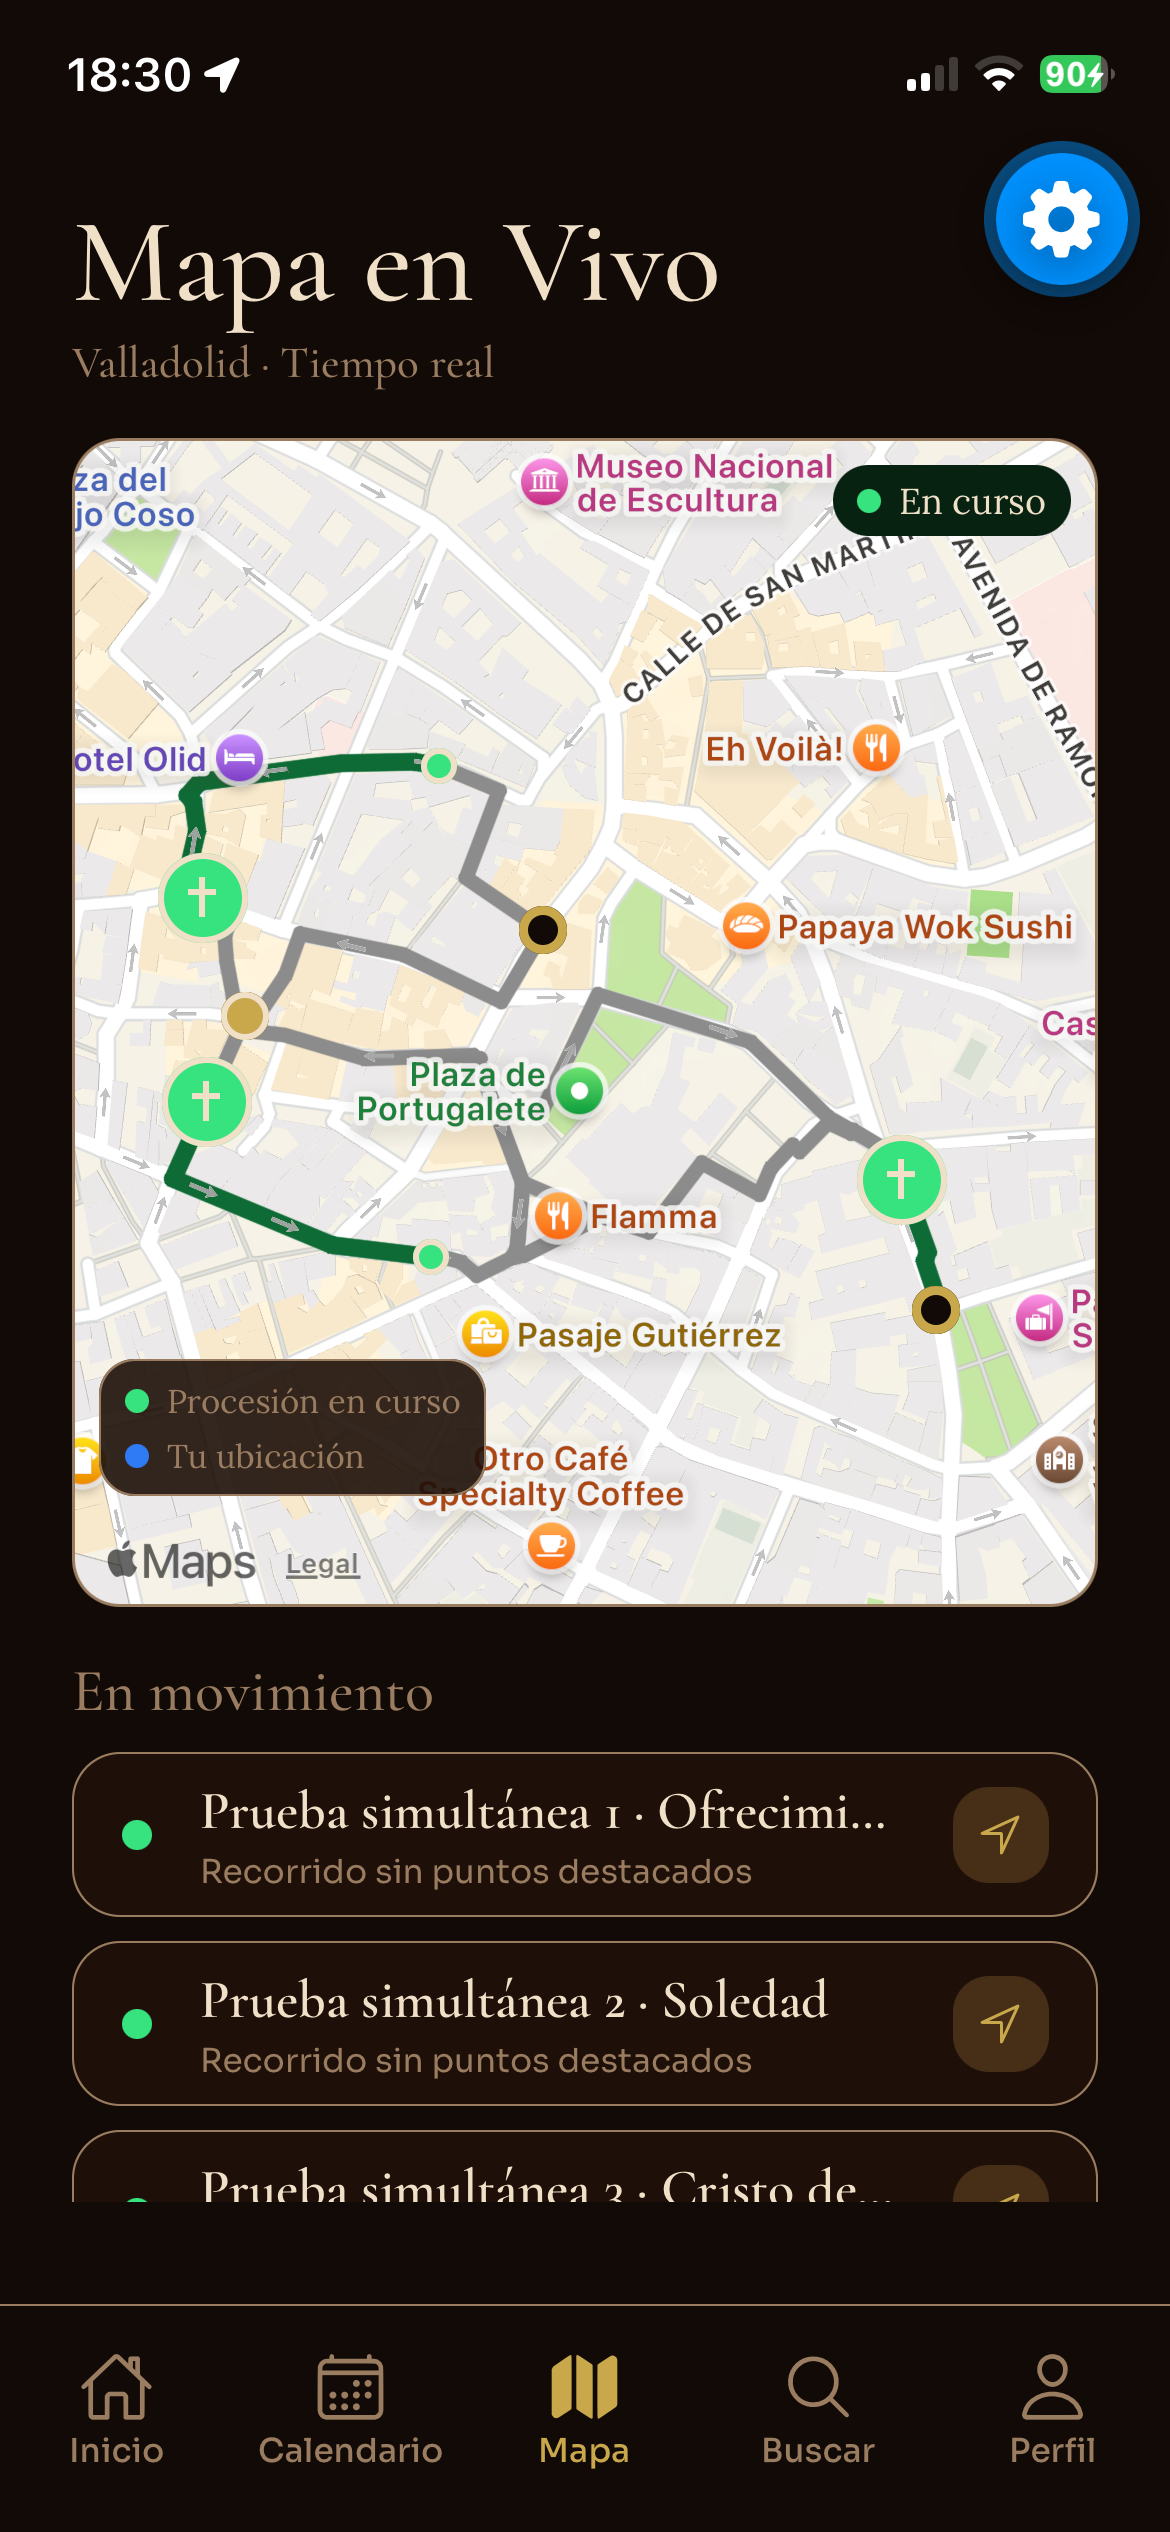
\includegraphics[width=\textwidth]{imagenes/mapa_variasProcesiones.PNG}
        \caption{Mapa en Vivo}
    \end{subfigure}
    \caption{Las tres procesiones de prueba en curso a la vez}
    \label{fig:pruebaVariasProcesiones}
\end{figure}

\begin{figure}[H]
    \centering
    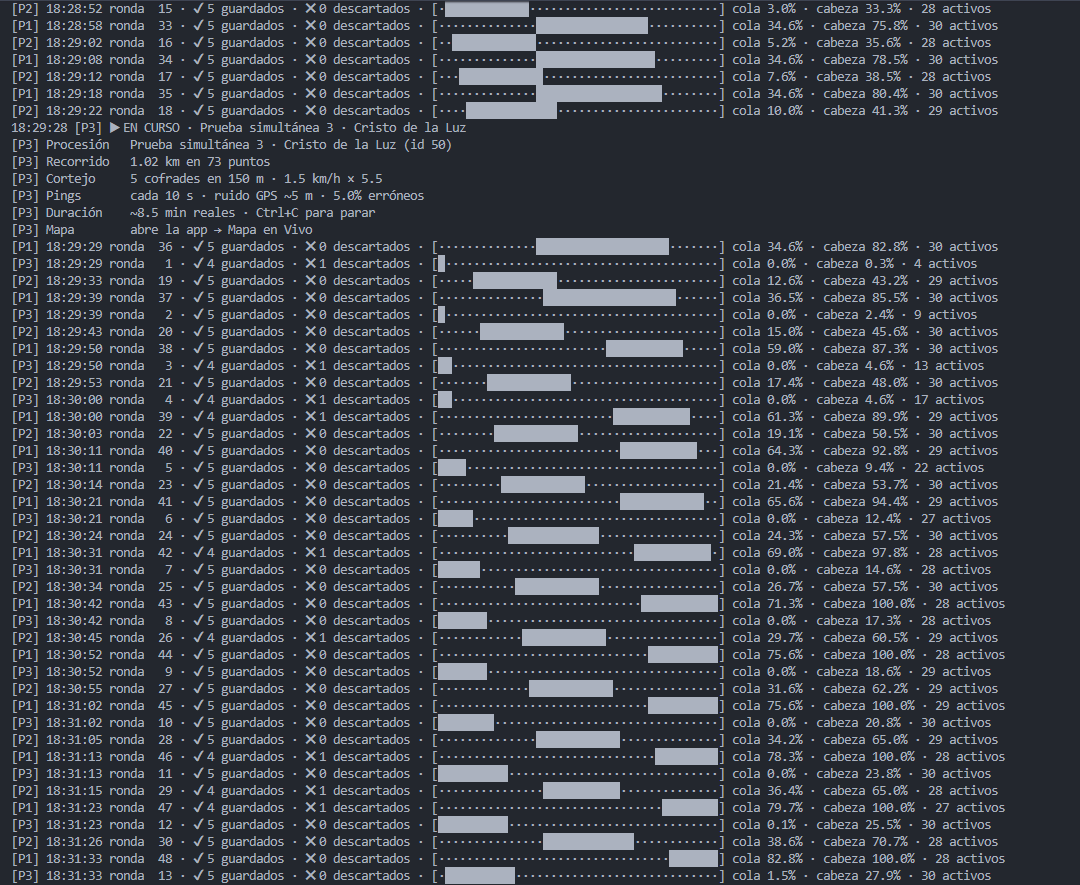
\includegraphics[width=\textwidth]{imagenes/consola_tresprocesiones_recortada.png}
    \caption{Salida de \texttt{prueba-varias.mjs} con las tres procesiones en curso}
    \label{fig:consolaVariasProcesiones}
\end{figure}


\section{Pruebas manuales de aceptación}\label{sec:pruebasAceptacion}

Por último, se ha recorrido cada caso de uso (Sección~\ref{cap:casos_de_uso} y Apéndice~\ref{cap:casos_de_uso_adicionales}) sobre la aplicación, en Android y en iOS, con cada uno de los cuatro roles, comprobando la secuencia base y las secuencias alternativas. La Tabla~\ref{tab:pruebasAceptacion} resume las pruebas agrupadas por rol.

\begin{table}[H]
\centering
\small
\renewcommand{\arraystretch}{1.2}
\begin{tabular}{|p{2.6cm}|p{8.6cm}|p{2.6cm}|}
\hline
\textbf{Rol} & \textbf{Casos de uso probados} & \textbf{Resultado} \\
\hline
Ciudadano & Seleccionar ciudad (con y sin permiso de ubicación), consultar información, listados, búsqueda y filtros, calendario, favoritos, estado de las notificaciones y Mapa en Vivo. & Superada \\
\hline
Cofrade & Iniciar sesión escaneando el QR y escribiendo el código, compartir ubicación (con la aplicación abierta y con la pantalla bloqueada), elegir procesión en curso y dejar de compartir. & Superada \\
\hline
Miembro de la Junta & Iniciar sesión, cambiar la contraseña provisional, solicitar la reactivación, gestionar cofradías, pasos, eventos y procesiones, importar el GPX, marcar puntos de interés, asignar pasos, crear notificaciones y gestionar los códigos QR. & Superada \\
\hline
Administrador & Gestionar ciudades, Juntas y miembros, reenviar la invitación, gestionar las solicitudes de reactivación y el propio perfil. & Superada \\
\hline
\end{tabular}
\caption{Pruebas manuales de aceptación}
\label{tab:pruebasAceptacion}
\end{table}

Las capturas de cada pantalla de la aplicación se recogen en el apartado de implementación de la iteración en la que se desarrolló (Capítulo~\ref{cap:iteraciones}). Como ejemplo de las pruebas del rol de cofrade, la Figura~\ref{fig:cofradeComparte} muestra la pantalla del cofrade compartiendo su ubicación en una de las procesiones de prueba. Al ejecutarse en Expo Go, que no permite la ubicación en segundo plano, la aplicación avisa de que solo se compartirá mientras esté abierta.

\begin{figure}[H]
    \centering
    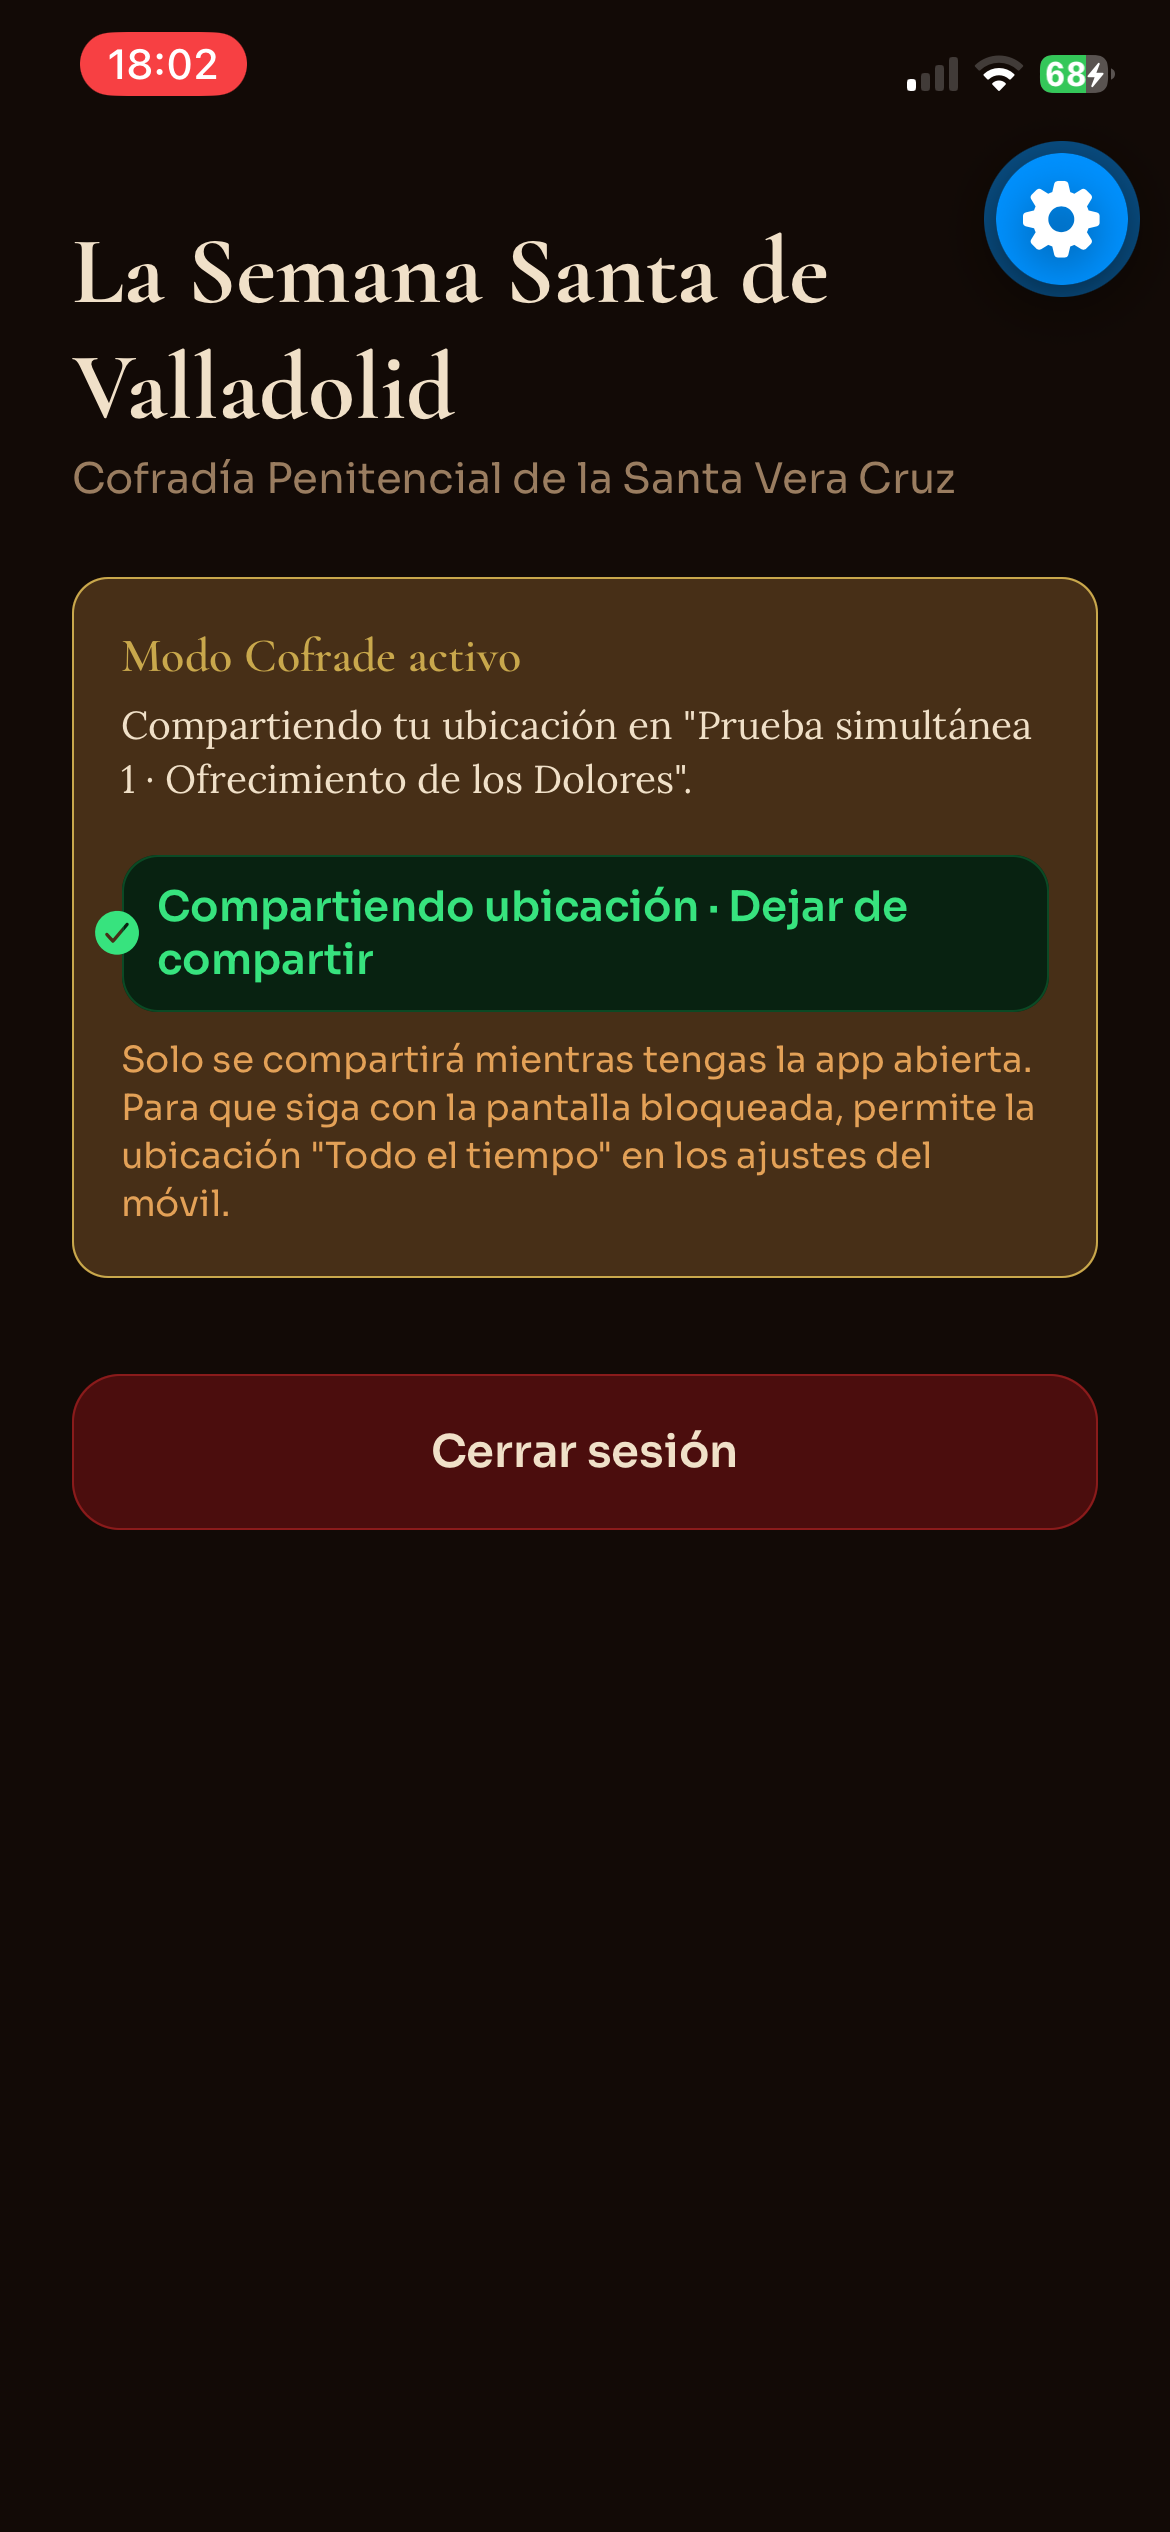
\includegraphics[width=0.35\textwidth]{imagenes/cofrade_comparte_ubicacion.PNG}
    \caption{Cofrade compartiendo su ubicación durante una procesión de prueba}
    \label{fig:cofradeComparte}
\end{figure}

\section{Errores detectados y corregidos}\label{sec:erroresDetectados}

Los errores encontrados durante las pruebas se han registrado en un documento del repositorio (\texttt{bugs.md}), con su prioridad, la causa, la solución aplicada y, cuando procede, la prueba automática que lo comprueba. En total se registraron 45 errores, de los que la gran mayoría están corregidos. Entre los más relevantes:

\begin{itemize}
    \item \textbf{Fallos de autorización}: cualquier usuario con sesión podía eliminar administradores; una Junta desactivada seguía pudiendo modificar datos; una Junta podía editar recorridos y ubicaciones de otra ciudad; y un código de acceso revocado seguía sirviendo hasta que caducaba la sesión del cofrade. Todos se corrigieron en el backend y se añadieron pruebas automáticas que los comprueban.
    \item \textbf{Seguimiento en tiempo real}: el cofrade dejaba de enviar su ubicación al bloquear el móvil, lo que se resolvió con una tarea en segundo plano; en los recorridos que salen y vuelven al mismo templo la estela aparecía completa desde la salida; solo se mostraba una procesión en curso aunque hubiera varias; y el cofrade no recibía ningún aviso cuando sus ubicaciones se descartaban por estar fuera del recorrido.
    \item \textbf{Integridad de los datos}: editar una procesión con varias cofradías dejaba solo una y borraba su templo de salida, y eliminar un elemento con datos asociados fallaba sin explicar el motivo.
\end{itemize}

Los errores que quedan pendientes son de prioridad media o baja y se recogen como trabajo futuro (Sección~\ref{cap:trabajo_futuro}): el envío de notificaciones a más de 100 dispositivos de una misma ciudad, la consulta sin conexión del detalle de procesiones y eventos, la representación de los puntos de interés en el mapa y la limitación de intentos al introducir un código de acceso.
